Our last topic is \emph{randomised linear algebra}: how can we incorporate random matrices into developing better algorithms for linear algebra?

\href{https://www.cambridge.org/core/services/aop-cambridge-core/content/view/4486926746CFF4547F42A2996C7DC09C/S0962492920000021a.pdf/div-class-title-randomized-numerical-linear-algebra-foundations-and-algorithms-div.pdf}{Martinsson \& Tropp 2020}

\section{Randomised trace estimation}
We begin with a simple question: can we compute the trace of a matrix without computing all the entries on the diagonal? Often one has a matrix $A \ensuremath{\in} \ensuremath{\bbR}^{n \ensuremath{\times} n}$ that we know how to compute matrix-vector $A\ensuremath{\bm{\x}}$, lets say in $O(n^2)$ operations, but we do not have direct access to the entries of the matrix $a_{kj}$. Of course, we can deduce the entries of a matrix via $a_{kj} = \ensuremath{\bm{\e}}_k^\ensuremath{\top} (A \ensuremath{\bm{\e}}_j)$, and hence we can compute the trace via:
\[
\Tr A = \ensuremath{\sum}_{k=1}^n a_{kk} = \ensuremath{\sum}_{k=1}^n \ensuremath{\bm{\e}}_k^\ensuremath{\top} A \ensuremath{\bm{\e}}_k,
\]
but this takes $O(n^3)$ operations. 

By the cyclic property of trace we have
\[
\Tr A = \Tr Q^\ensuremath{\top} A Q = \ensuremath{\sum}_{k=1}^n \ensuremath{\bm{\q}}_k^\ensuremath{\top} A \ensuremath{\bm{\q}}_j
\]
for any orthogonal matrix $Q$. Let's do an experiment where we take a fixed matrix $A$:


\begin{lstlisting}
0.9303525062438385
\end{lstlisting}


\section{Least squares}
We begin with an introduction to least squares.  For a rectangular matrix $A \ensuremath{\in} \ensuremath{\bbR}^{m \ensuremath{\times} n}$ with $m > n$ and a right-hand side $\ensuremath{\bm{\b}} \ensuremath{\in} \ensuremath{\bbR}^m$ we cannot solve $A \ensuremath{\bm{\c}} = \ensuremath{\bm{\b}}$ unless $\ensuremath{\bm{\b}}$ happens to be in the column span of $A$. However, we can instead find $\ensuremath{\bm{\c}} \ensuremath{\in} \ensuremath{\bbR}^n$ that satisfies $A \ensuremath{\bm{\c}} \ensuremath{\approx} \ensuremath{\bm{\b}}$, in the sense that
\[
\| A\ensuremath{\bm{\c}} - \ensuremath{\bm{\b}}\|
\]
is minimised. This is called the \emph{least squares} solution.  Minimising a norm is equivalent to minimising its square, and expanding out we see that it is equivalent to a quadratic minimisation problem:
\[
\| A\ensuremath{\bm{\c}} - \ensuremath{\bm{\b}}\|^2 = (A\ensuremath{\bm{\c}} - \ensuremath{\bm{\b}})^\ensuremath{\top} (A\ensuremath{\bm{\c}} - \ensuremath{\bm{\b}}) = \ensuremath{\bm{\c}}^\ensuremath{\top} A^\ensuremath{\top} A \ensuremath{\bm{\c}} - 2 \ensuremath{\bm{\c}}^\ensuremath{\top} A^\ensuremath{\top} \ensuremath{\bm{\b}}  + \ensuremath{\bm{\b}}^\ensuremath{\top} \ensuremath{\bm{\b}}.
\]
In the scalar case ($n = 1$ so that $\ensuremath{\bm{\c}}$ is essentially a constant) we know we can solve this by differentiation with respect to $\ensuremath{\bm{\c}}$, and we arrive at a linear system
\[
 A^\ensuremath{\top} A \ensuremath{\bm{\c}}  =  A^\ensuremath{\top} \ensuremath{\bm{\b}}
\]
This generalises (after some linear algebra) and in general we have that
\[
\ensuremath{\bm{\c}} =  (A^\ensuremath{\top} A)^{-1} A^\ensuremath{\top} \ensuremath{\bm{\b}}.
\]
A classic application of least squares is \emph{polynomial regression}. In the case of linear regression, we want to approximation data $\{b_j\}$ on a grid of points $\{x_j\}$ by a linear function $c_0 + c_1 x$. In other words, we want to solve
\[
\underbrace{\begin{bmatrix} 1 & x_1 \\
1 & x_2 \\
\ensuremath{\vdots} & \ensuremath{\vdots} \\
1 & x_n
\end{bmatrix}}_A \underbrace{\begin{bmatrix} c_0 \\
c_1
\end{bmatrix}}_{\ensuremath{\bm{\c}}} \ensuremath{\approx} \underbrace{\begin{bmatrix}
b_1 \\
b_2 \\
\ensuremath{\vdots} \\
b_n
\end{bmatrix}}_{\ensuremath{\bm{\b}}}
\]
by using the least squares solution.

Here is a depiction of $c_0 + c_1 x$, which is the least squares fit at  the (noisy) data at $n = 50$ points:


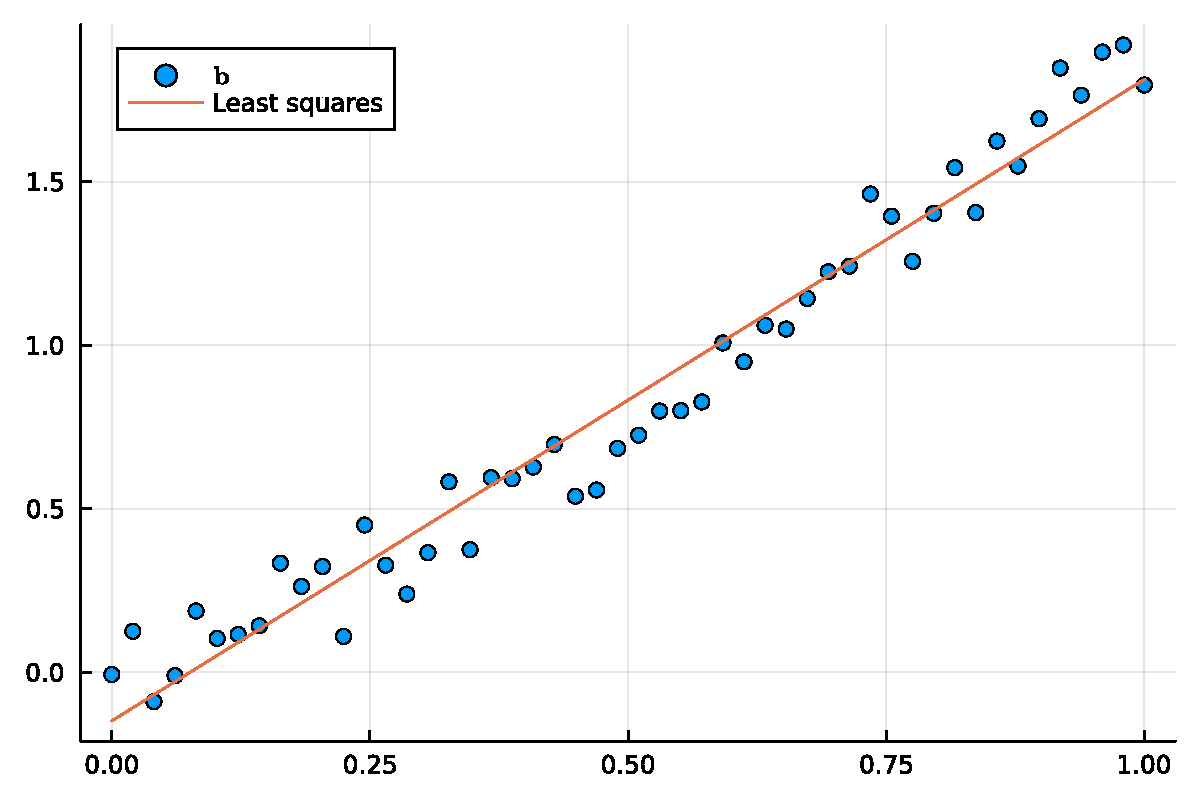
\includegraphics[width=0.6\linewidth,height=0.45\linewidth]{figures/III.RandomisedLinearAlgebra_2_1.pdf}

\section{Randomised least squares}
In the above  data there is a lot of correlation between nearby points, hence, using every single point is unnecessary. An alternative is to \emph{sketch} the problem: use a sketch matrix $P \ensuremath{\in} \ensuremath{\bbR}^{r \ensuremath{\times} m}$ where $r \ensuremath{\ll} m$ and solve
\[
P A \ensuremath{\bm{\c}} \ensuremath{\approx} P \ensuremath{\bm{\b}}
\]
using least squares. Here we see a simple example where we use $P \ensuremath{\in} \ensuremath{\bbR}^{5 \ensuremath{\times} 50}$ with random entries:


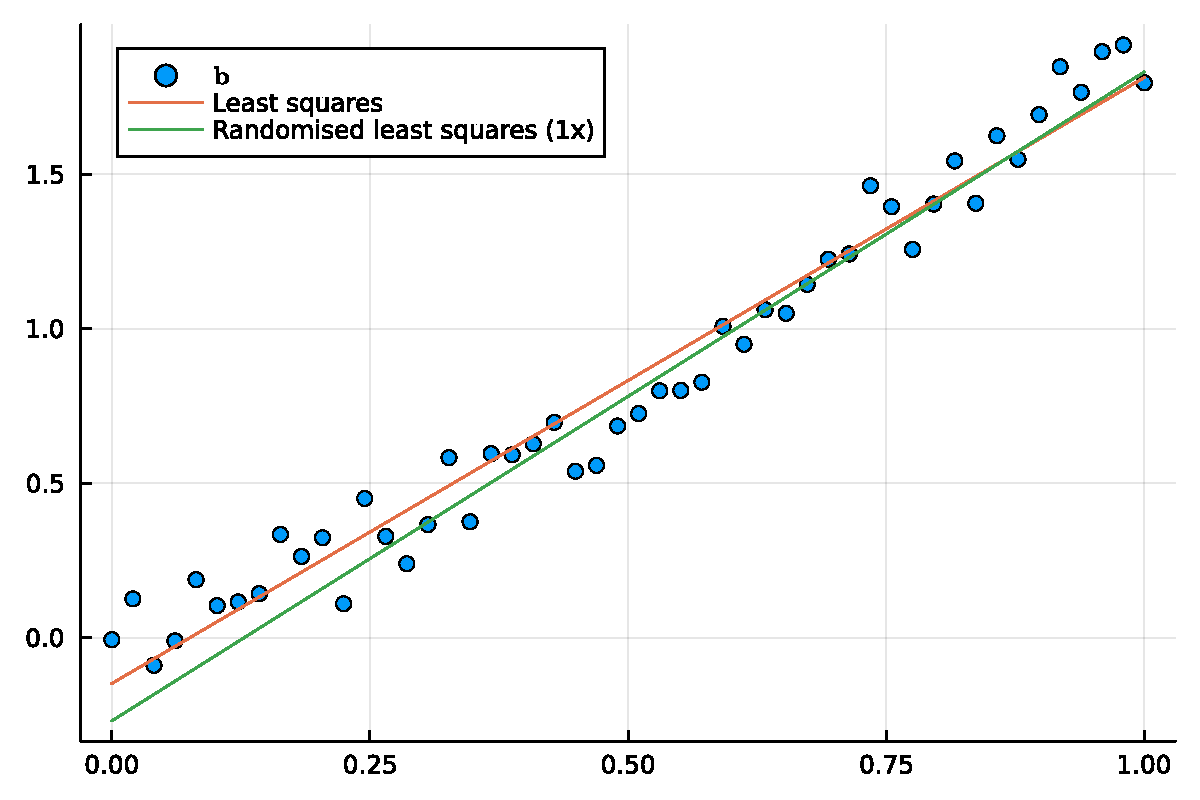
\includegraphics[width=0.6\linewidth,height=0.45\linewidth]{figures/III.RandomisedLinearAlgebra_3_1.pdf}

This is a single sample and, to the eye, it performs equally well as least squares. Going further, we see that averaging over multiple trials is almost indistiguishable from the true least squares approximation:


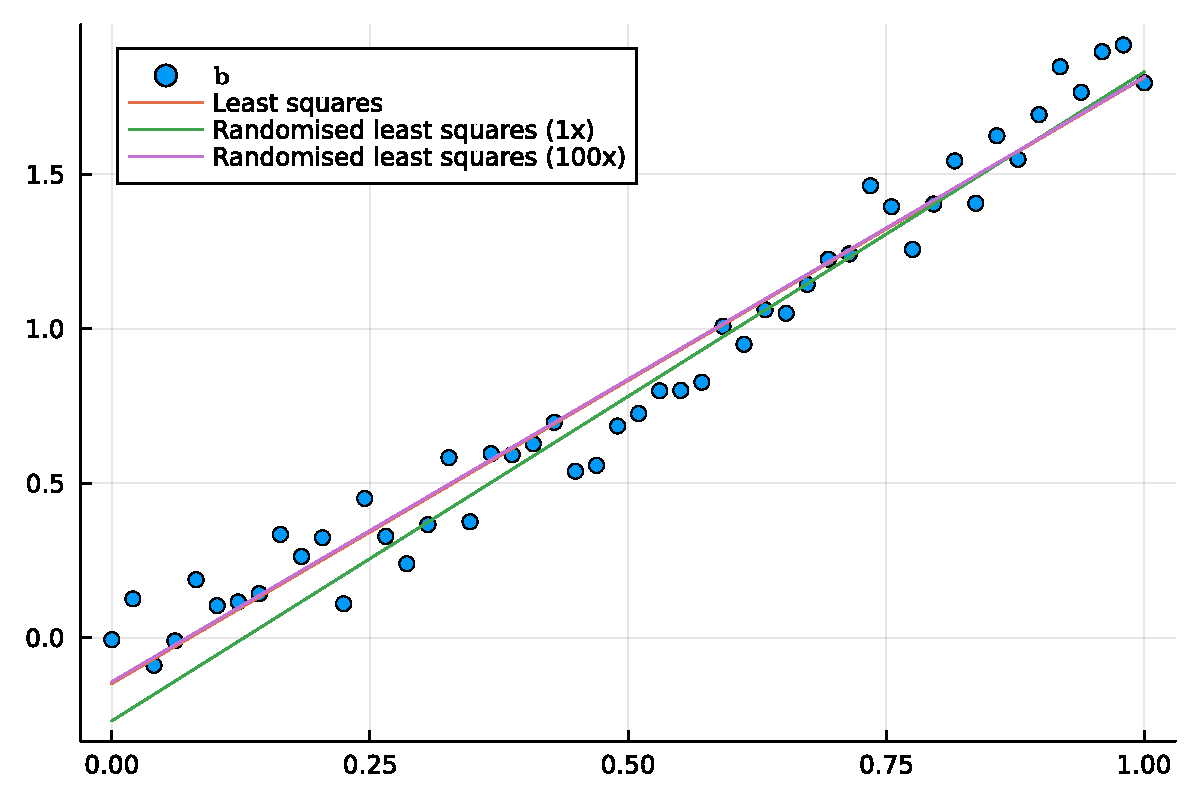
\includegraphics[width=0.6\linewidth,height=0.45\linewidth]{figures/III.RandomisedLinearAlgebra_4_1.pdf}

Now this particular example is a bit silly: its not at all clear that solving 100 least squares systems of size $5 \ensuremath{\times} 2$ is preferred to a single least squares system of size $50 \ensuremath{\times} 2$. But we can consider a much more extreme example of $n = 10,000$. Here we compare the average over samples for varying $r$:


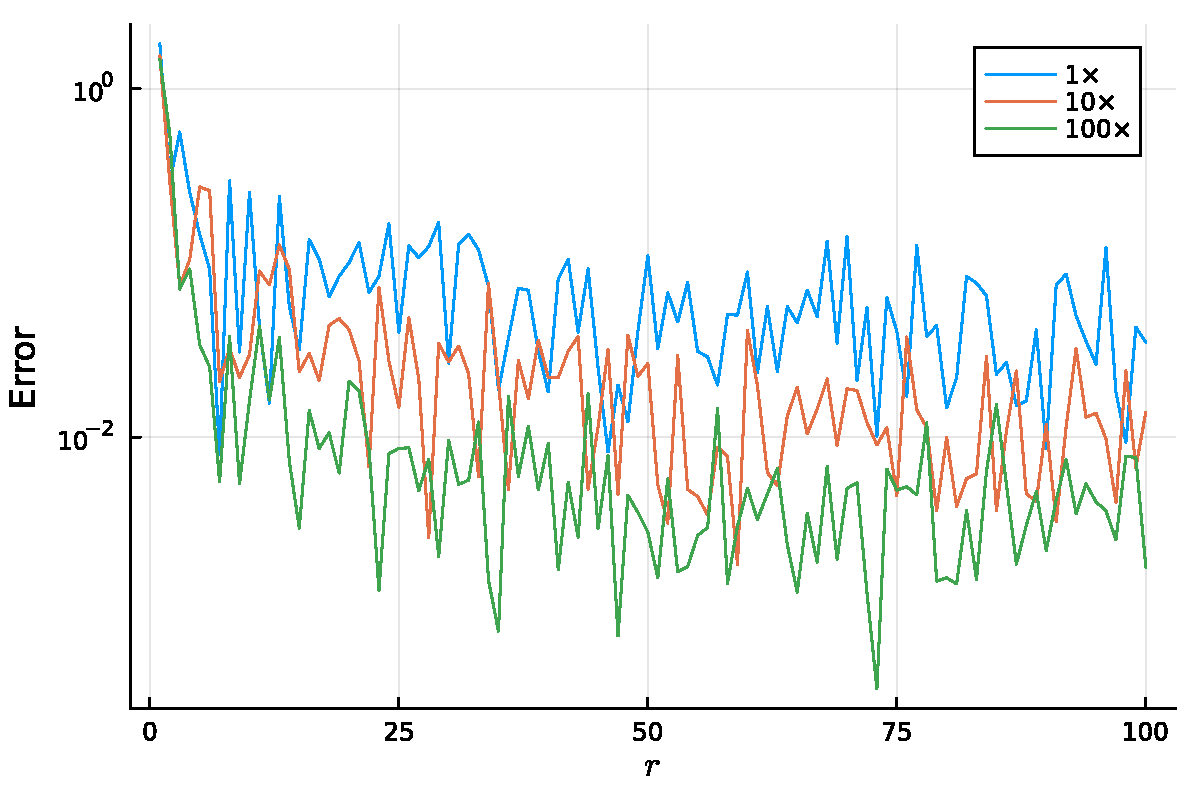
\includegraphics[width=0.6\linewidth,height=0.45\linewidth]{figures/III.RandomisedLinearAlgebra_5_1.pdf}

That is to say, we can achieve accuracy to within about $1\%$ by solving 100 least squares problems involving $10 \ensuremath{\times} 2$ matrices.

\section{Poster projects}
\begin{itemize}
\item[1. ] How does the approximation property depend on the distribution of the sketch matrix?


\item[2. ] What other algorithms are amenable to randomisation (low rank approximation, norm estimation, multiplication)?


\item[3. ] Can averaging over multiple sketch matrices be used to improve accuracy while preserving speed advantage?


\item[4. ] What applications are there to randomised linear algebra such as regression?

\end{itemize}

